%-------------------------------------------------------------------------------
%   Haskellerのための圏論 - 圏
%   Keichi
%   圏論の勉強成果の個人的なまとめ
%-------------------------------------------------------------------------------

%-------------------------------------------------------------------------------
\section{圏}

\subsection{定義}
ある圏(Category)$C$は、2つの集合の組からなる:

\begin{itemize}
    \item $Ob(C)$、$C$の「対象」(Object)の集合
    \item $Ar(C)$、$C$の「射」(Morphism)の集合
\end{itemize}

$Ar(C)$に含まれる射$f$は、$Ob(C)$の要素であるドメイン(Domain)
(もしくはソース(Source))$dom f$と、コドメイン(Codomain)(もしくはターゲット(Target))
$cod f$を持つ。$f:A \to B$と書けば、fのドメインが$A$であり、コドメインが
$B$であることを意味する。

\begin{figure}[htbp]
    \centering
    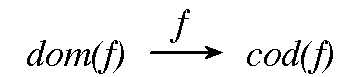
\includegraphics{diag_dom.pdf}
    \caption{ドメインとコドメイン}
\end{figure}

また合成という操作が存在し、これは$\circ$と表記される。
例えば、射$g \circ f$が定義されるとき、$f$のコドメインは$g$のドメインと等しく、
$g \circ f$のドメインとコドメインはそれぞれ$f$のドメインと$g$のコドメイン
となる。つまり、射$f$と$g$が存在し、$f:A \to B$かつ$g:B \to C$ならば、
$g \circ f = A \to C$ということである。また、ある対象$A$について、
$id_A: A \to A$という射が定義される。これは恒等射と呼ばれ、
$id$とだけ表記されることも多い。

\begin{figure}[htbp]
    \centering
    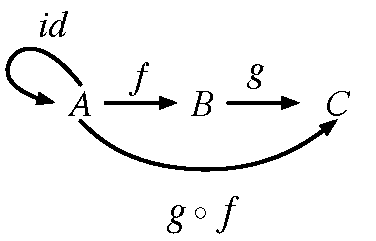
\includegraphics{diag_comp.pdf}
    \caption{恒等射と合成}
\end{figure}

また、圏$C$においてHomset集合を
$hom_C(A,B)=\{f \mid f \in Ar(C), f: A \to B\}$と定義する。
これはつまり、圏$C$において対象$A$から$B$への射の集合である。

\subsection{公理}
また、$C$が圏であるためには、以下の条件が満たされている必要がある:
\begin{itemize}
    \item $f:A \to B$なら$f \circ id_A = id_b \circ f = f$
        (恒等射は左単位元、右単位元である)
    \item $f:A \to B$かつ$g: B \to C$か$h: B \to D$なら、
        $h \circ (g \circ f)=(h\circ g) \circ f$(射は結合律を満たす)
\end{itemize}

\subsection{圏の例}
\begin{itemize}
    \item Set, 集合を対象とし、集合間の写像を射とする
    \item Mon, モノイドを対象とし、モノイドの射を射とする
        (モノイドは対象が1つだけの圏ともとらえれる)
    \item Grp, 群を対象とし、群の準同型写像を射とする
    \item Hask, Haskellの型を対象とし、関数を射とする圏
    \item Cat, 圏を対象とし、関手を射とする圏の圏
    \item 関数を対象とし、データの流れを射とする圏(データフローダイアグラム)
\end{itemize}

\subsection{Haskellでの例}
Haskellの型と関数からなる圏Haskを考えると、
圏Haskの対象$Ob(Hask)$は全てのHaskellの型の集合、
\[\{Int, Bool, Float, String, \ldots\}\]
である。また、$Ar(Hask)$は全てのHaskellの関数の集合、
\[\{(+), length, even, \ldots\}\]
となる。圏Haskにおいて射の合成$\circ$は、関数合成演算子
\begin{lstlisting}
    (.)::(b->c)->(a->b)->(a->c)
\end{lstlisting}
であり、恒等射は恒等関数
\begin{lstlisting}
   id::a->a
\end{lstlisting}
となる。単位元律および結合律が成り立つのは明らかである。(seqなどの例外はあるが)

%-------------------------------------------------------------------------------
